%%%%%%%%%%%%%%%%%%%%%%%%%%%%%%%%%%%%%%%%%%%
%                                         %
% This file should only be made of \input %
%                                         %
%%%%%%%%%%%%%%%%%%%%%%%%%%%%%%%%%%%%%%%%%%%

\chapter{Le client}

	\paragraph{}La partie client de notre application sert à interagir avec 
l'utilisateur humain. Basiquement, l'utilisateur tape des commandes et le 
client lui renvoie un résultat généré par le daemon.
	
	\section{Architecture logique du client}

La figure \ref{client} illustre l'architecture de notre client. Tout d'abord, 
le client se charge de créer une socket permettant de se connecter à son daemon
, avec l'IP et le port adéquat. Il crée ensuite un thread qui s'occupe de gérer
 l'envoi des commandes tapées par l'utilisateur, en exécutant la fonction 
\verb"send_cmd()". Cette fonction crée elle aussi un thread qui, par le biais 
de la fonction \verb"recv_resp()", s'occupe d'afficher à l'écran les réponses 
aux commandes reçues du daemon.

\begin{center}
\begin{figure}[H]
    \centering
    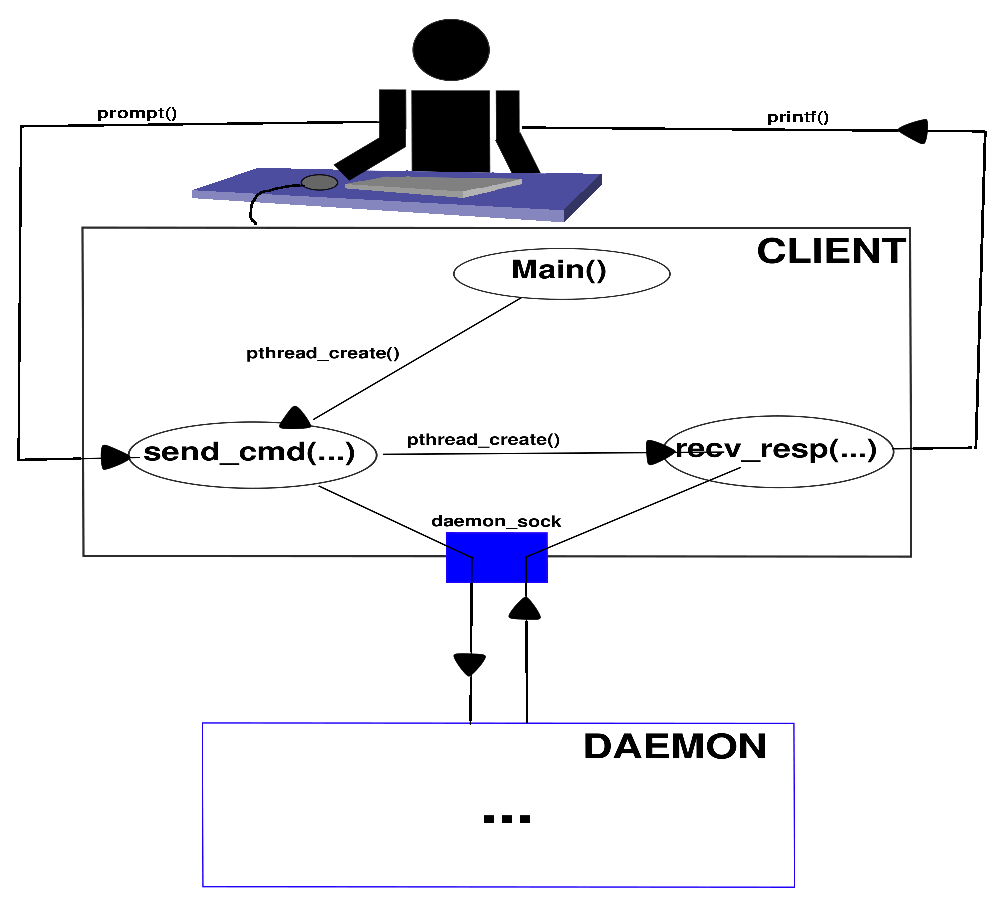
\includegraphics[scale=0.95]{client/archi_client.eps}
    \caption{Architecture du client}
    \label{client}
\end{figure}
\end{center}
	
	\section{Gestion des requ\^etes}

Le client s'occupe uniquement de renvoyer à l'utilisateur les réponses reçues
du daemon. En conséquence, l'intégralité des requêtes utilisateurs ne sont pas 
gérées directement par la partie client de notre application, mais par le 
daemon. Voir la partie \ref{protclient}.
	
